
\chapter[Dạng bài: Xác định thời điểm, số lần gặp nhau trong một khoảng thời gian của hai vật trong dao động điều hòa;\\
Bài tập: Xác định thời điểm, số lần gặp nhau của hai vật trong dao động điều hòa]{Dạng bài: Xác định thời điểm, số lần gặp nhau trong một khoảng thời gian của hai vật trong dao động điều hòa;\\Bài tập: Xác định thời điểm, số lần gặp nhau của hai vật trong dao động điều hòa}
\section{Lý thuyết}
\subsection{Hai vật dao động điều hòa cùng tần số, khác biên độ}
Biểu diễn hai vật dao động điều hòa cùng tần số, khác biên độ bằng hai đường tròn đồng tâm (hình vẽ).

Khi gặp nhau thì hình chiếu của hai vectơ quay $\overrightarrow{\text{OM}}$, $\overrightarrow{\text{ON}}$ trên trục hoành trùng nhau. Khi đó MN vuông góc với trục $\text{O}x$.

\begin{center}
	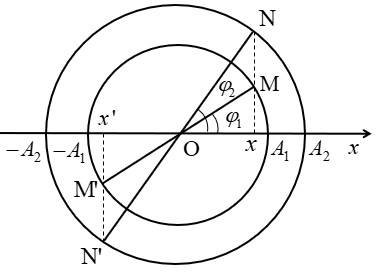
\includegraphics[scale=0.8]{../figs/VN12-PH-02-A-001-5-V2-1.jpg}
\end{center}

Dựa vòng tròn lượng giác ta nhận thấy rằng cứ sau khoảng thời gian $\dfrac{T}{2}$ thì $\triangle\text{MON}$ lại có cạnh MN vuông góc với $\text{O}x$.\\
Vậy khoảng thời gian ngắn nhất giữa hai lần mà hai vật gặp nhau là $\dfrac{T}{2}$.

Số lần hai vật gặp nhau tính theo công thức
\begin{equation*}
	n=\left[\dfrac{t}{0,5T}\right],
\end{equation*}
với $[\ ]$ là kí hiệu của phép lấy phần nguyên.

\luuy{Cần xem xét lúc $t=0$ thì hai vật có gặp nhau hay không.}
\subsection{Hai vật dao động điều hòa cùng biên độ, khác tần số}
Hai vật trong dao động điều hòa khác tần số, cùng biên độ có phương trình là
\begin{equation*}
	x_1=A\cos(\omega_1 t+\varphi_1)
\end{equation*}
và 
\begin{equation*}
	x_2=A\cos(\omega_2 t+\varphi_2).
\end{equation*}
Hai vật gặp nhau khi chúng có cùng li độ:
$$x_1=x_2.$$
Giải phương trình trên, ta tìm được $t$ là thời điểm gặp nhau.
\section{Mục tiêu bài học - Ví dụ minh họa}
\begin{dang}{Sử dụng được phương trình dao động\\ và đường tròn lượng giác để xác định\\ thời điểm hai vật gặp nhau}
	\ppgiai{
		\begin{description}
			\item[Bước 1:] Xác định vị trí, thời điểm gặp nhau lần đầu $t_1$.
			\item[Bước 2:]  Thời điểm gặp nhau lần thứ $n$ $t = (n-1)\cdot\dfrac{T}{2} + t_1$ với ($n=1,2,3,...$).
		\end{description}
	}
	\viduii{3}{Hai vật dao động điều hòa dọc theo trục song song với nhau. Phương trình dao động của các vật lần lượt là $x_1 =3\cos \left(5\pi t - \dfrac{\pi}{3}\right)$; $x_2 =2\sqrt 3\cos \left(5\pi t -\dfrac{\pi}{2}\right)$ ($x$ tính bằng cm, $t$ tính bằng giây). Thời điểm gặp nhau lần đầu tiên của hai vật có giá trị gần giá trị nào nhất sau đây?
		\begin{mcq}(4)
			\item $\SI{0,067}{s}$.
			\item $\SI{0,3}{s}$.
			\item $\SI{0,15}{s}$.
			\item $\SI{0,5}{s}$.
		\end{mcq}
	}
	{\begin{center}
			\textbf{Hướng dẫn giải}
		\end{center}
		
		Khi gặp nhau thì $x_1=x_2$, suy ra
		
		\begin{equation*}
			3\cos \left(5\pi t - \dfrac{\pi}{3}\right) = 2\sqrt 3\cos \left(5\pi t -\dfrac{\pi}{2}\right).
		\end{equation*}
		\begin{equation*}
			\Rightarrow 3\cos \left(5\pi t - \dfrac{\pi}{3}\right) = 2\sqrt 3\cos \left(5\pi t -\dfrac{\pi}{3}- \dfrac{\pi}{6}\right).
		\end{equation*}
		Đặt $y=5\pi t -\dfrac{\pi}{3}$ ta có phương trình:
		\begin{equation*}
			3\cos y =2\sqrt 3 \cos \left(y -\dfrac{\pi}{6}\right)
		\end{equation*}
		\begin{equation*}
			\Rightarrow 3\cos y =2\sqrt 3 \left (\cos y \cos \dfrac{\pi}{6}+ \sin y \sin \dfrac{\pi}{6}\right)
		\end{equation*}
		\begin{equation*}
			\Rightarrow	3\cos y =3\cos y +\sqrt 3 \sin y
		\end{equation*}
		\begin{equation*}
			\Rightarrow \sin y =0 \Leftrightarrow y =k\pi.
		\end{equation*}
		\begin{equation*}
			\Rightarrow y =5\pi t -\dfrac{\pi}{3} =k\pi
		\end{equation*}
		\begin{equation*}
			\Rightarrow t =\dfrac{1}{15} + \dfrac{k}{5}; k =0,1,2,...
		\end{equation*}
		Thời điểm gặp nhau đầu liên ứng với $k=0$, ta được $t=\dfrac{1}{15}\approx \SI{0,067}{s}$.
		
		\textbf{Đáp án: A.}
	}
	\viduii{3}{Hai chất điểm cùng thực hiện dao động điều hòa trên cùng một trục $\text{O}x$ có cùng biên độ nhưng tần số lần lượt là $f_1=\SI{3}{\hertz}$ và $f_2=\SI{6}{\hertz}$. Lúc đầu cả hai chất điểm đều qua li độ ${A}/{2}$ theo chiều dương. Thời điểm đầu tiên ngay sau đó mà các chất điểm gặp nhau lần nữa là
		\begin{mcq}(4)
			\item $\dfrac{2}{27}\ \text{s}$.
			\item $\dfrac{1}{3}\ \text{s}$.
			\item $\dfrac{1}{9}\ \text{s}$.
			\item $\dfrac{1}{27}\ \text{s}$.
		\end{mcq}
	}
	{\begin{center}
			\textbf{Hướng dẫn giải}
		\end{center}
		
		Tần số góc dao động của vật 1 là
		\begin{equation*}
			\omega_1=2\pi f_1=2\pi\cdot\SI{3}{\hertz}=6\pi\,\text{rad/s}.
		\end{equation*}
		
		Tần số góc dao động của vật 2 là
		\begin{equation*}
			\omega_2=2\pi f_2=2\pi\cdot\SI{6}{\hertz}=12\pi\,\text{rad/s}.
		\end{equation*}
		
		Lúc đầu cả hai chất điểm đều qua li độ $\dfrac{A}{2}$ theo chiều dương nên
		\begin{equation*}
			\cos\varphi=\dfrac{1}{2}\Rightarrow\varphi=-\dfrac{\pi}{3}.
		\end{equation*}
		
		Phương trình dao động của vật 1 là
		\begin{equation*}
			x_1=A\cos(6\pi t-\dfrac{\pi}{3}).
		\end{equation*}
		
		Phương trình dao động của vật 2 là
		\begin{equation*}
			x_2=A\cos(12\pi t-\dfrac{\pi}{3}).
		\end{equation*}
		
		Hai vật gặp nhau khi chúng có cùng li độ
		\begin{eqnarray*}
			&&x_1=x_2\\
			&\Leftrightarrow&\cos(6\pi t-\dfrac{\pi}{3})=\cos(12\pi t-\dfrac{\pi}{3})\\
			&\Leftrightarrow&
			\begin{cases}
				6\pi t-\dfrac{\pi}{3}=12\pi t-\dfrac{\pi}{3}+k2\pi\\
				6\pi t-\dfrac{\pi}{3}=-12\pi t+\dfrac{\pi}{3}+k2\pi
			\end{cases}\\
			&\Leftrightarrow&
			\begin{cases}
				t=-\dfrac{k}{3}\\
				t=\dfrac{1}{27}+\dfrac{k}{9}.
			\end{cases}
		\end{eqnarray*}
		
		Thời điểm 2 vật gặp nhau là $t=\dfrac{1}{27}+\dfrac{k}{9}$ với $k=0,1,2,3,...$
		
		Thời điểm gặp nhau lần đầu tiên tương ứng với $k=0$, ta được $t=\dfrac{1}{27}\,\text{s}$.
		
		\textbf{Đáp án: D.}
	}
	
\end{dang}
\begin{dang}{Sử dụng được phương trình dao động\\ và đường tròn lượng giác để xác định\\ số lần hai vật gặp nhau}
	\ppgiai{
		\begin{description}
			\item[Bước 1:] Kiểm tra xem lúc $t=0$ chúng có cùng vị trí hay không.
			\item[Bước 2:] Xác định số lần hai vật gặp nhau.
			\begin{itemize}
				\item Nếu ban đầu hai vật khác vị trí, số lần hai vật gặp nhau bằng \textbf{phần nguyên} của $t$ chia nửa chu kì $T$ là
				\begin{equation*}
					n=\left[\dfrac{t}{0,5T}\right].
				\end{equation*}
				\item Nếu ban đầu hai vật cùng vị trí, số lần hai vật gặp nhau là $n+1$.
			\end{itemize}
		\end{description}
		\luuy{Cần kiểm tra xem lúc $t=0$ chúng có cùng vị trí hay không, nếu cùng vị trí và tính cả lần đó thì số lần sẽ là $n+1$.}
	}
	\viduii{3}{Hai vật dao động điều hòa dọc theo các trục song song với nhau. Phương trình dao động của các vật lần lượt là
		$x_1=3\cos\left(5\pi t-\dfrac{\pi}{3}\right)$ và $x_2=\sqrt{3}\cos\left(5\pi t-\dfrac{\pi}{6}\right)$
		($x$ tính bằng cm, $t$ tính bằng s). Trong khoảng thời gian $\SI{1}{\second}$ đầu tiên thì hai vật gặp nhau mấy lần? 
		\begin{mcq}(4)
			\item 5 lần.
			\item 6 lần.
			\item 7 lần.
			\item 8 lần.
		\end{mcq}
		
	}
	{\begin{center}
			\textbf{Hướng dẫn giải}
		\end{center}
		
		Tại thời điểm ban đầu $(t=0)$ ta có $x_1=x_2=\dfrac{3}{2}\ \text{cm}$.
		
		Chu kì dao động của hai vật:
		\begin{equation*}
			T=\dfrac{2\pi}{\omega}=\dfrac{2\pi}{5\pi\,\text{rad/s}}=\SI{0,4}{\second}.
		\end{equation*}
		
		Số lần hai vật gặp nhau trong $\SI{1}{\second}$ đầu tiên là
		\begin{equation*}
			n=\left[\dfrac{t}{0,5T}\right]+1=\left[\dfrac{1}{0,5\cdot0,4}\right]+1=5+1=6.
		\end{equation*}
		
		\textbf{Đáp án: B.}
	}
	
	\viduii{3}{Hai vật dao động điều hòa với cùng biên độ $A$, tần số lần lượt là là $f_1=\SI{3}{\hertz}$ và $f_2=\SI{6}{\hertz}$. Lúc đầu hai vật xuất phát từ vị trí có li độ $\dfrac{A\sqrt 3}{2}$. Khoảng thời gian ngắn nhất để hai vật có cùng li độ là
		\begin{mcq}(4)
			\item $\dfrac{1}{27}\ \text{s}$.
			\item $\dfrac{1}{36}\ \text{s}$.
			\item $\dfrac{2}{27}\ \text{s}$.
			\item $\dfrac{1}{54}\ \text{s}$.
		\end{mcq}
		
	}
	{\begin{center}
			\textbf{Hướng dẫn giải}
		\end{center}
		
		Phương trình dao động của vật 1:
		\begin{equation*}
			x_1 =A \cos \left(6\pi t -\dfrac{\pi}{6}\right)\ \text{cm}.
		\end{equation*}
		Phương trình dao động của vật 2:
		\begin{equation*}
			x_2 =A \cos \left(12\pi t -\dfrac{\pi}{6}\right)\ \text{cm}.
		\end{equation*}
		Hai vật gặp nhau khi $x_1=x_2$, suy ra
		\begin{equation*}
			\cos \left(6\pi t -\dfrac{\pi}{6}\right) - \cos \left(12\pi t -\dfrac{\pi}{6}\right) =0.
		\end{equation*}
		\begin{equation*}
			\Leftrightarrow \sin 3\pi t \cdot \sin \left(9\pi t -\dfrac{\pi}{6}\right) = 0.
		\end{equation*}
		\begin{equation*}
			\Leftrightarrow 9\pi t -\dfrac{\pi}{6} =k\pi
		\end{equation*}
		\begin{equation*}
			\Rightarrow t=\dfrac{k\pi + \dfrac{\pi}{6}}{9\pi}
			\Rightarrow t_\text{k=0} = \dfrac{1}{54}\ \text{s}.
		\end{equation*}
		
		Vậy khoảng thời gian ngắn nhất để hai vật có cùng li độ là $\dfrac{1}{54}\ \text{s}$
		
		\textbf{Đáp án: D.}
	}
\end{dang}